\documentclass[a4paper, 12pt]{article}
\usepackage[T1]{fontenc}
\usepackage[utf8]{inputenc}
\usepackage[polish]{babel}
\usepackage{polski}
\usepackage{times}
\usepackage{geometry}
\geometry{a4paper, margin=1in}
\usepackage{hyperref}
\usepackage{bookmark} % Add this line
\usepackage{titling}
\usepackage{graphicx} % Add this line

\title{
    \begin{minipage}{0.4\textwidth}
        
\includegraphics[height=30px]{logoPWR.png} % Change the height to 30px
    \end{minipage}
    \hfill
    \begin{minipage}{0.4\textwidth}
        \raggedleft
        
\includegraphics[height=30px]{image.png} % Change the height to 30px
    \end{minipage}
    \vspace{2cm} % Adjust the space between the logos and the title
    \\
    Sprawozdanie z Laboratoriumnr 2\\ 
    \large Przedmiotu  Grafika komputerowa
    i komunikacja człowiek-komputer\\ 
    \small Temat: Podstawy OpenGL\\
}
\author{Kyrylo Semenchenko 273004 \\
Informatyka Techniczna I stopnia \\
Wydział Informatyki i Telekomunikacji}
\date{\today}

\begin{document}

\maketitle

\tableofcontents

\newpage

\section{Wstęp}

W ramach drugiego laboratorium należało:
\begin{itemize}
    \item Zapoznać się z podstawowymi elementami grafiki komputerowej,
    \item Zrozumieć proces powstawania obrazu w komputerze,
    \item Oswoić się z interfejsem OpenGL na przykładach 2D.
\end{itemize}

Do realizacji tych celów przygotowano środowisko pracy w wybranym języku programowania -- Pythonie. Pobrano niezbędne biblioteki, a także przykładowy program. Następnie przystąpiono do wykonywania zadań.

\section{Wykonane zadania}

\subsection{Zadanie 1}

Należało:
\begin{itemize}
    \item Przerobić kod,
    \item Narysować trójkąt, w którym każdy wierzchołek ma inny kolor,
    \item Pamiętać o ustawionych parametrach rzutni:
    \begin{itemize}
        \item Zakres na osi X: od -100.0 (lewa strona) do 100.0 (prawa strona),
        \item Zakres na osi Y: od -100.0 (dół okna) do 100.0 (góra okna),
        \item Punkt o współrzędnych (X = 0, Y = 0) znajduje się w środku okna.
    \end{itemize}
\end{itemize}

Wynik renderowania pierwszego kodu przedstawiono na \hyperref[fig:zad1]{Rysunku 1}.

\begin{figure}[h]
    \centering
    \begin{minipage}{0.45\textwidth}
        \centering
        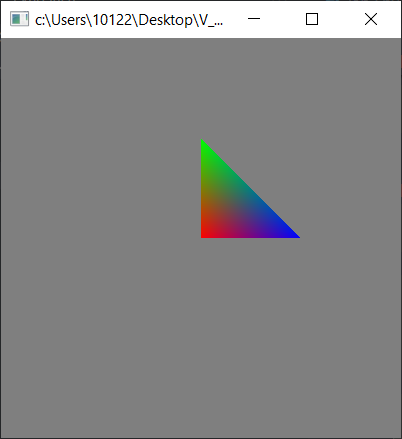
\includegraphics[width=\textwidth]{zad1.png}
        \caption{Renderowanie trójkąta z kolorowymi wierzchołkami.} 
        \label{fig:zad1}
    \end{minipage}
    \hfill
    \begin{minipage}{0.45\textwidth}
        \centering
        \label{fig:zad2}
        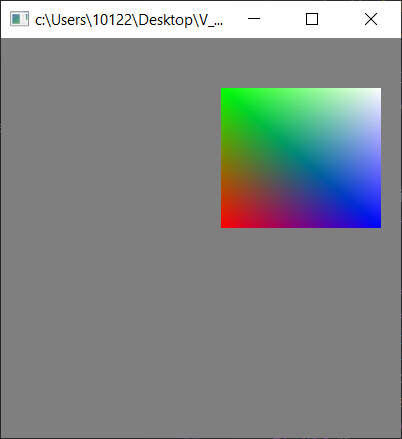
\includegraphics[width=\textwidth]{zad2.png}
        \caption{Renderowanie prostokąta z kolorowymi wierzchołkami.}
    \end{minipage}
\end{figure}
\subsection{Zadanie 2}

Należało:
\begin{itemize}
    \item Dodać nową funkcję, która przyjmuje cztery argumenty:
    \begin{itemize}
        \item Położenie na osi X -- \texttt{x},
        \item Położenie na osi Y -- \texttt{y},
        \item Rozmiar pierwszego boku -- \texttt{a},
        \item Rozmiar drugiego boku -- \texttt{b}.
    \end{itemize}
    \item Położenie (\texttt{x}, \texttt{y}) może wskazywać środek prostokąta lub jego wierzchołek. Punkt (\texttt{x}, \texttt{y}) określa się fachowo jako \textit{punkt początkowy} (ang. \textit{origin point}).
    \item Na tej podstawie należy wyznaczyć współrzędne reszty wierzchołków bryły.
    \item Do narysowania prostokąta należy wykorzystać dokładnie dwa trójkąty.
    \item Funkcję należy wywołać przykładowo w ramach \texttt{render()}.
\end{itemize}

Wynik renderowania kodu przedstawiono na \hyperref[fig:zad2]{Rysunku 2}.

\subsection{Zadanie 3}

Należało wprowadzić losowość kolorów i deformacje w prostokącie. Wskazówki:
\begin{itemize}
    \item Rozbudować funkcję z poprzedniego zadania, na przykład:
    \begin{itemize}
        \item Dodać kolejny argument do funkcji -- \texttt{d} -- z domyślną wartością 0.0,
        \item Nowy argument powinien sterować stopniem deformacji,
        \item Można przeskalować rozmiary boków \texttt{a} i \texttt{b}.
    \end{itemize}
    \item Uzyskać losową wartość w Pythonie:
    \begin{itemize}
        \item Załadować bibliotekę \texttt{random},
        \item Przykładowe wywołanie: \texttt{random.random()},
        \item Przydatne może być także użycie \texttt{random.seed(...)}.
    \end{itemize}
\end{itemize}

Wynik renderowania kodu pokazano na \hyperref[fig:zad3]{Rysunku 3}.

\begin{figure}[h]
    \centering
    \begin{minipage}[t]{0.4\textwidth}
        \centering
        \label{fig:zad3}
        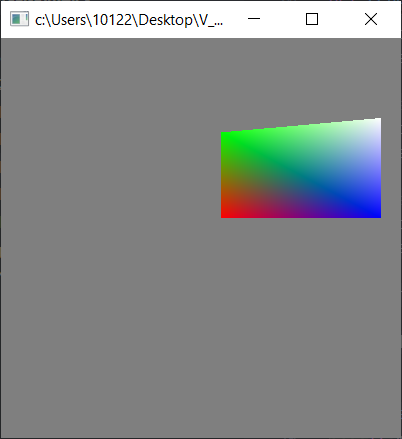
\includegraphics[height=0.25\textheight]{zad3.png}
        \caption{Renderowanie asymetrycznego prostokta z kolorowymi wierzchołkami.}
    \end{minipage}
    \hfill
    \begin{minipage}[t]{0.58\textwidth}
        \centering
        \label{fig:zad4}
        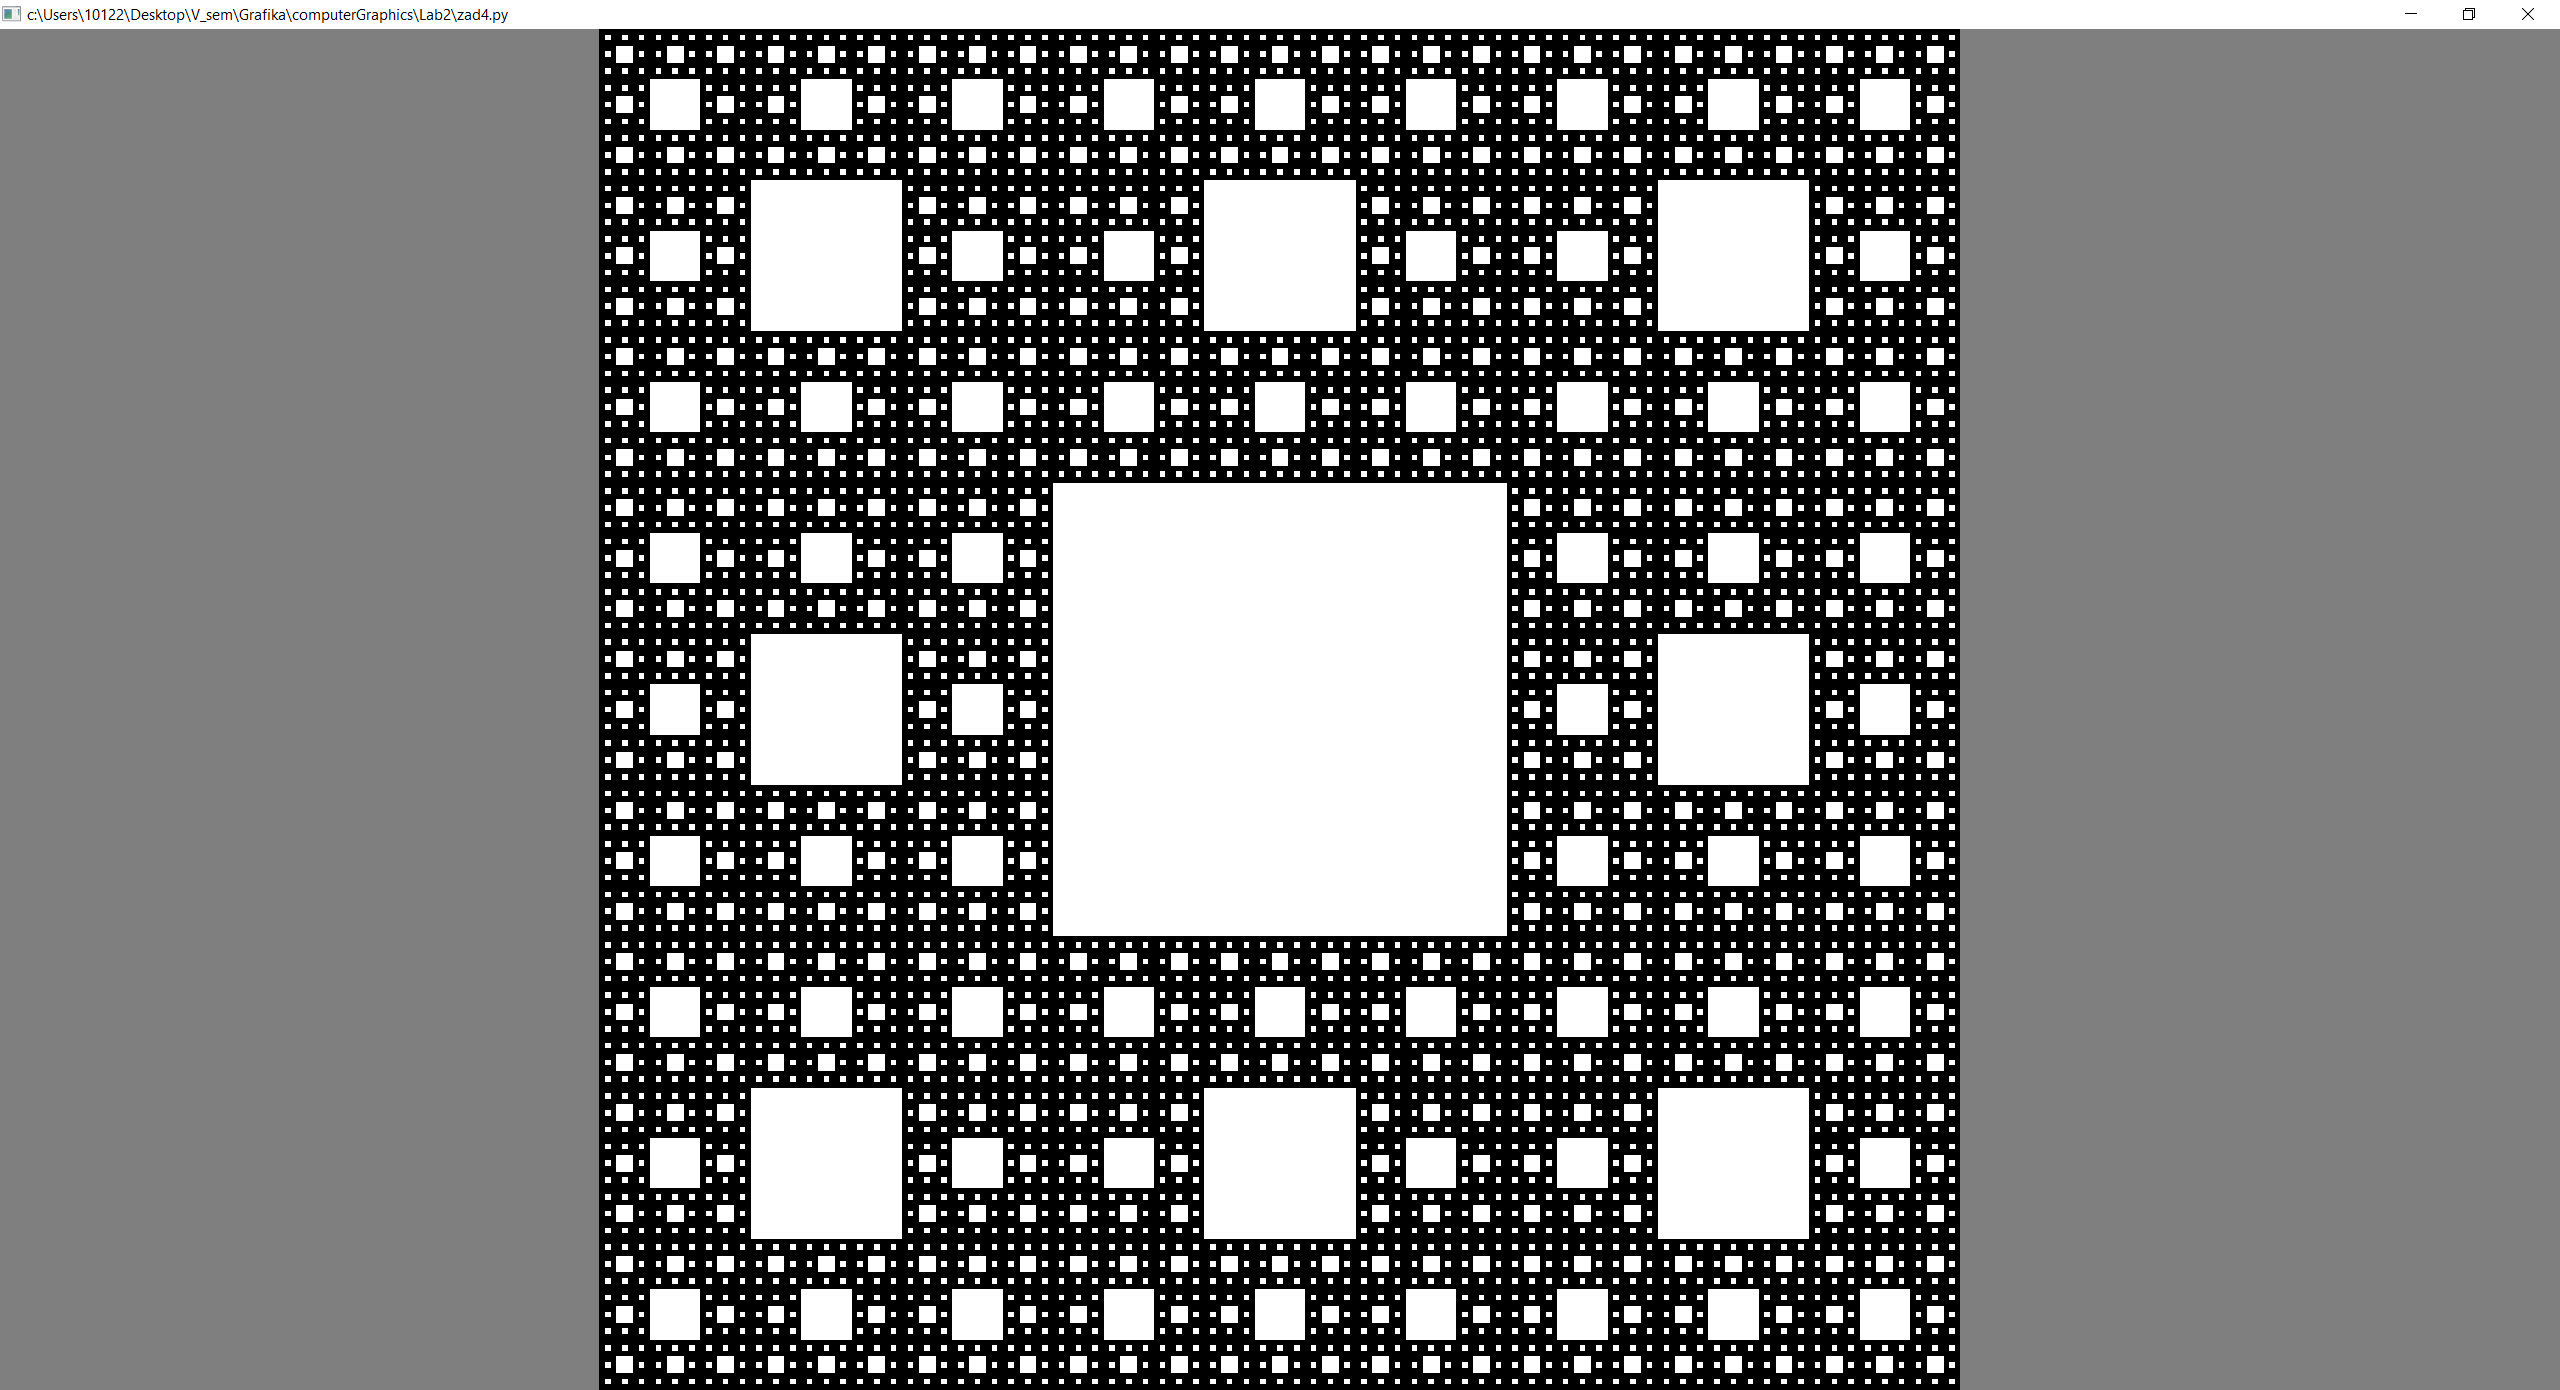
\includegraphics[height=0.25\textheight]{zad4.png}
        \caption{Fraktal rysowany przy użyciu rekurencji.}
    \end{minipage}
\end{figure}


\subsection{Zadanie 4}

Należało:
\begin{itemize}
    \item Istnieją dwa podejścia do narysowania tego fraktalu:
    \begin{itemize}
        \item Rysować poszczególne małe prostokąty w wyznaczonych miejscach.
        \item Narysować duży prostokąt i pomniejsze w miejscach "wycięć".
    \end{itemize}
    \item Wykorzystać funkcje z poprzednich przykładów:
    \begin{itemize}
        \item Najpierw narysować zarys fraktalu z ręcznie rozmieszczonych brył, aby wyznaczyć współrzędne interesujących nas prostokątów.
        \item Następnie ubrać całość w funkcję rekurencyjną i powtórzyć rysowanie w wyznaczonych współrzędnych. Z każdym stopniem rekurencji pomniejszać rozmiary boków.
    \end{itemize}
    \item Stopień samopodobieństwa powinien być parametrem programu.
\end{itemize}

W tym zadaniu został zaimplementowany dywan Sierpińskiego (\textit{Sierpinski Carpet}) przy użyciu OpenGL, gdzie złożoność fraktalu jest kontrolowana przez parametr głębokości rekurencji.

\textbf{Opis algorytmu:}

\begin{itemize}
    \item Algorytm rekurencyjnie dzieli dany prostokąt na dziewięć równych mniejszych prostokątów.
    \item Prostokąt w centrum każdego podziału jest "wycięty" (pozostawiony biały), podczas gdy pozostałe są czarne.
    \item Z każdym kolejnym poziomem rekurencji rozmiary prostokątów są zmniejszane o jedną trzecią, a procedura jest powtarzana dla wszystkich mniejszych prostokątów oprócz środkowego.
\end{itemize}

\textbf{Główne elementy kodu:}

\begin{itemize}
    \item Funkcja \texttt{draw\_square} rysuje pojedynczy kwadrat o zadanej wielkości w odpowiednich współrzędnych.
    \item Funkcja \texttt{sierpinski\_carpet} wywołuje funkcję \texttt{draw\_square} rekurencyjnie, tworząc strukturę fraktala na podstawie aktualnych współrzędnych i głębokości.
    \item Program działa w oknie o rozmiarze 400x400 pikseli, gdzie parametr głębokości rekurencji jest pobierany od użytkownika.
\end{itemize}

Na Rysunku \hyperref[fig:zad4]{Rysunkku 4} przedstawiono renderowanie fraktala dywanu Sierpińskiego. Z każdym stopniem rekurencji zwiększa się liczba prostokątów, co prowadzi do bardziej złożonego wzoru. Algorytm generuje zróżnicowane struktury w zależności od głębokości rekurencji wybranej przez użytkownika.



\subsection{Zadanie 5 (zadanie domowe)}

Należało:
\begin{itemize}
    \item Wybrać jeden z przykładów zaproponowanych jako zadania domowe. Dokument znajduje się na stronie prowadzącego.
    \item Interesujące były pomysły na generację fraktali. Nie trzeba było implementować różnych wariantów tego samego fraktala.
\end{itemize}

Został wybrany fraktal plazmowy (\textit{plasma fractal}), a polecenie zostało wykonane na podstawie dostępnych materiałów.

\textbf{Opis algorytmu:}

Fraktal plazmowy został wygenerowany na podstawie metody podziału kwadratu, która działa rekurencyjnie:

\begin{itemize}
    \item Początkowy kwadrat jest podzielony na cztery mniejsze.
    \item Każdy wierzchołek kwadratu ma przypisany losowy kolor.
    \item Środkowy punkt kwadratu oblicza się jako średnią kolorów wierzchołków, z dodatkowym losowym przesunięciem, aby uzyskać efekt szumu.
    \item Algorytm jest powtarzany dla każdego z czterech nowych kwadratów, aż do osiągnięcia zadanego minimalnego rozmiaru.
\end{itemize}

\textbf{Główne elementy kodu:}

\begin{itemize}
    \item Funkcja \texttt{plasma} realizuje rekurencyjne podziały i oblicza kolory na podstawie wartości wierzchołków.
    \item Funkcja \texttt{render} odpowiada za rysowanie fraktala na ekranie poprzez kolejne wywołania funkcji \texttt{plasma}.
    \item Program tworzy okno o rozmiarze 400x400 pikseli, w którym fraktal jest dynamicznie rysowany.
\end{itemize}

Na \hyperref[fig:zad5]{Rysunkku 5} przedstawiono renderowanie fraktala plazmowego. Wygenerowany obraz ukazuje płynne przejścia kolorystyczne, które są efektem losowego szumu dodawanego do wartości kolorów wierzchołków kwadratów. Algorytm generuje zróżnicowane wzory w zależności od losowych wartości przypisywanych na każdym etapie rekurencji.

\begin{figure}[h]
    \centering
    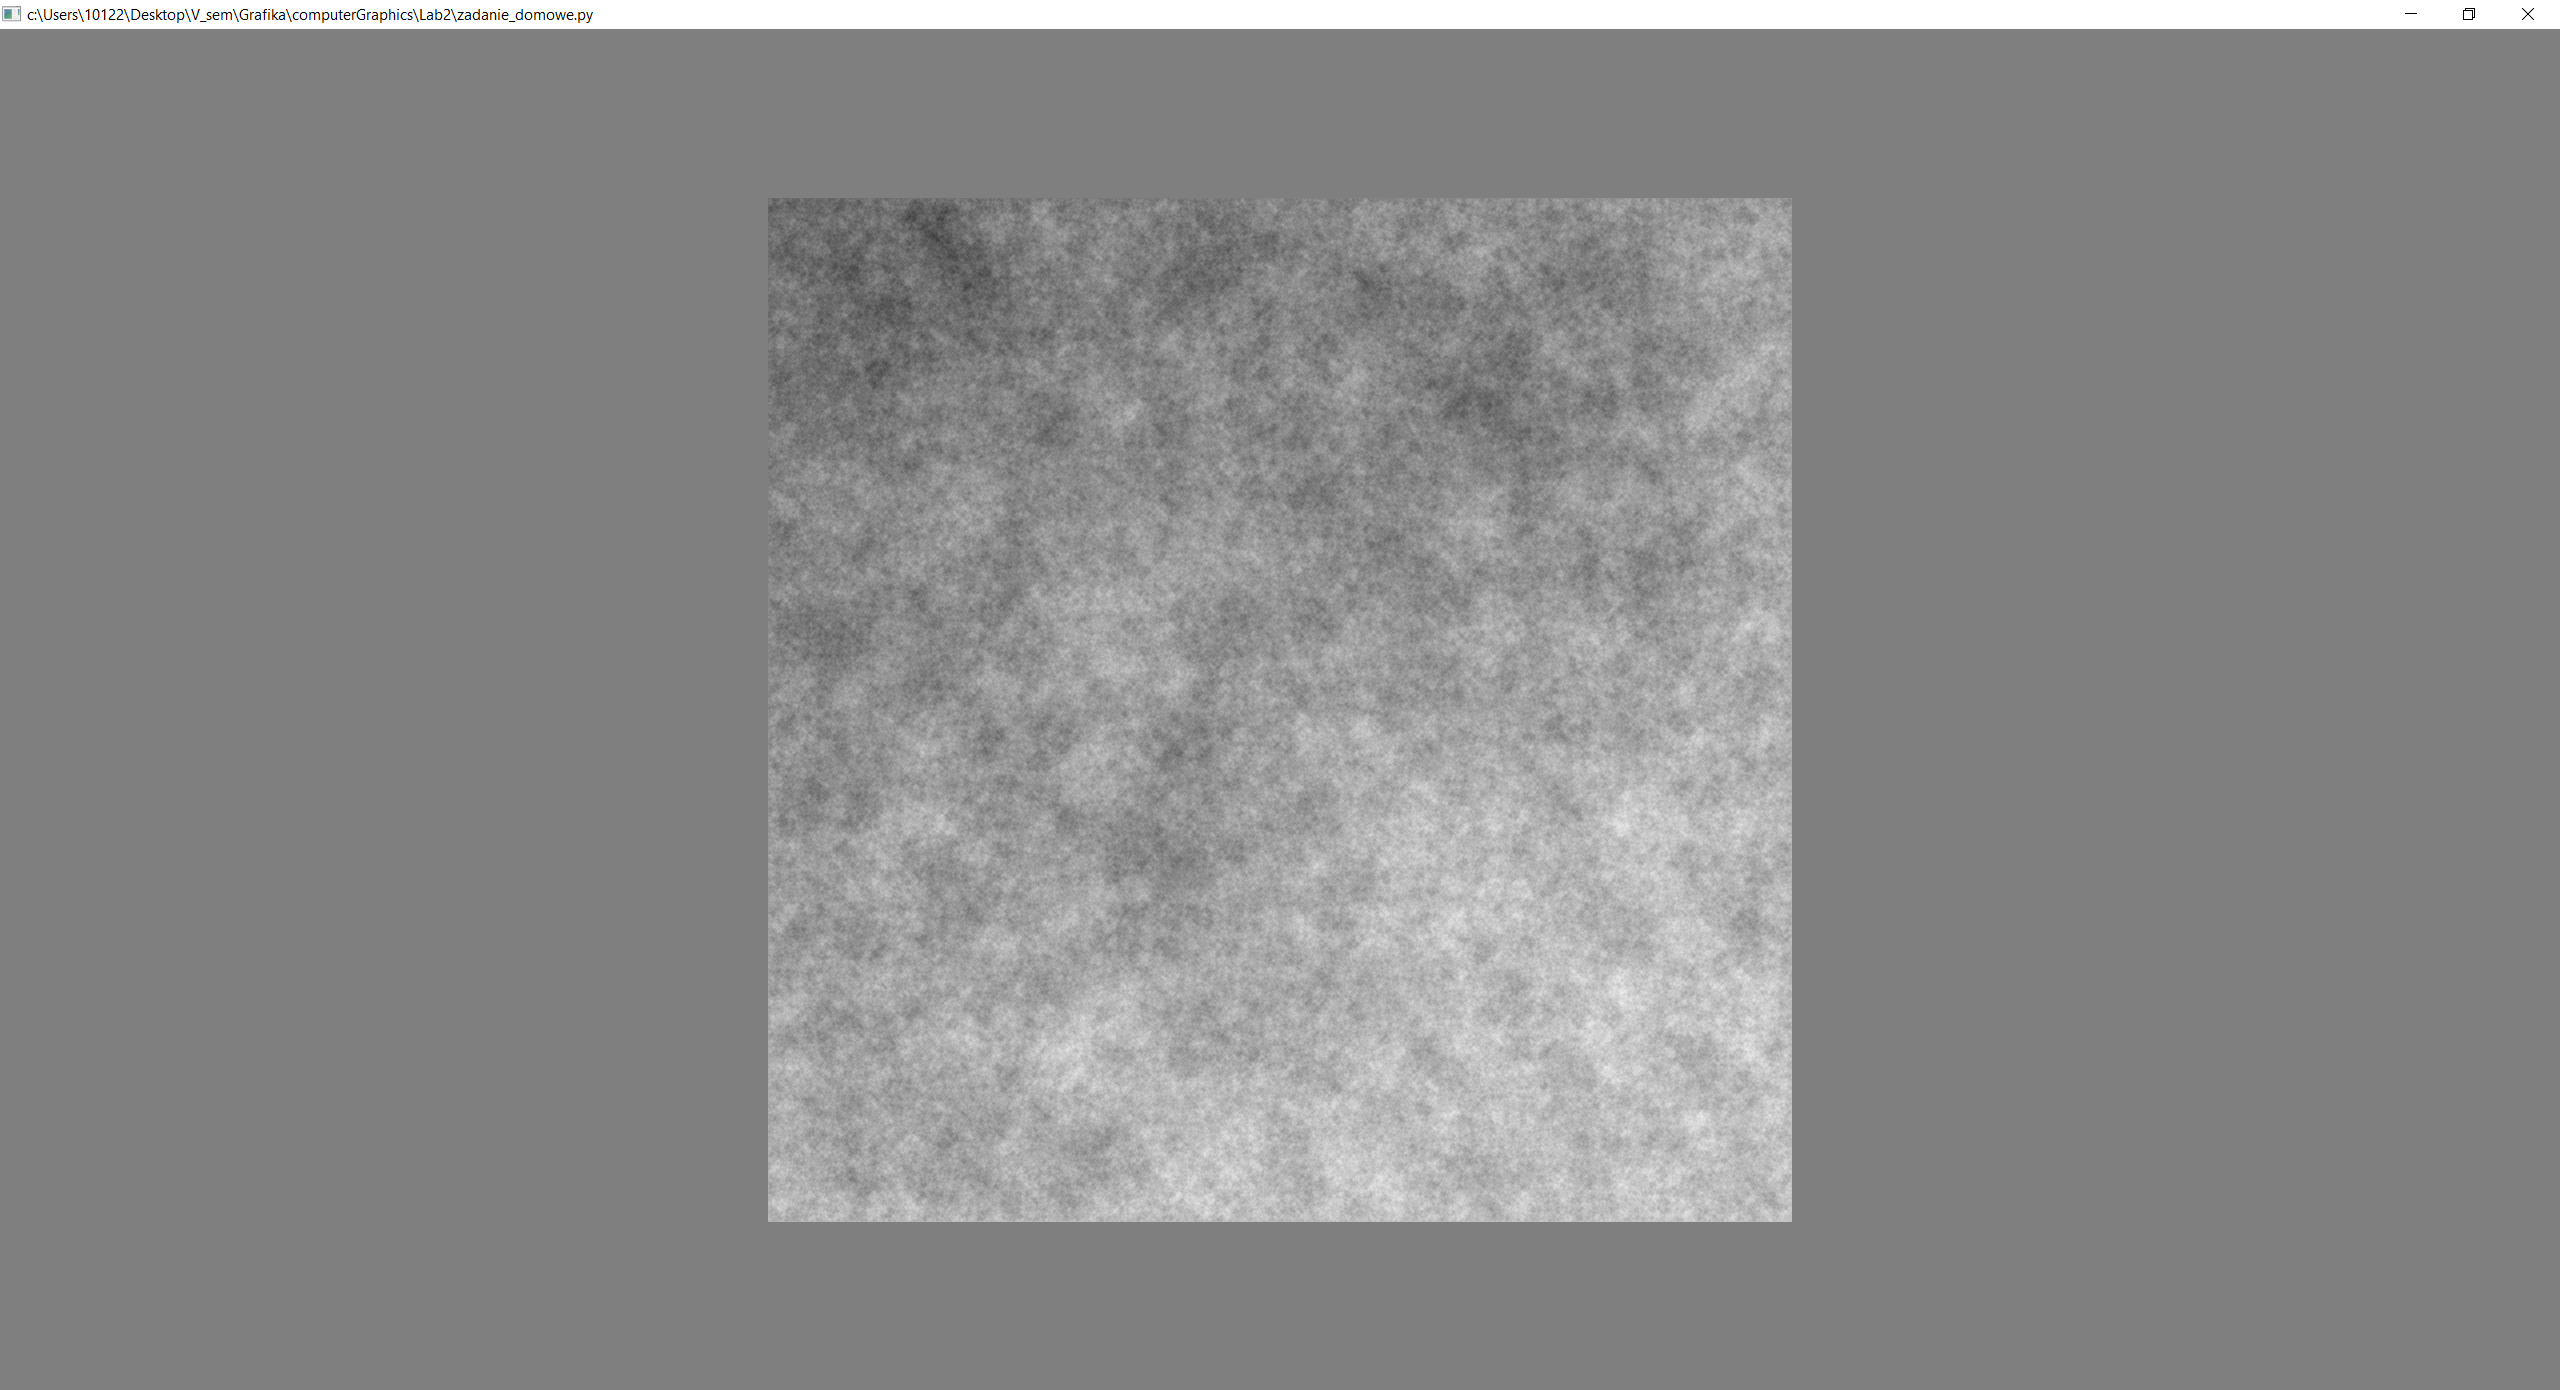
\includegraphics[width=0.98\textwidth]{zad5.png}
    \caption{Fraktal plazmowy.}
    \label{fig:zad5}
\end{figure}

\end{document}